% This LaTeX was auto-generated from MATLAB code.
% To make changes, update the MATLAB code and export to LaTeX again.

\documentclass{article}

\usepackage[utf8]{inputenc}
\usepackage[T1]{fontenc}
\usepackage{lmodern}
\usepackage{graphicx}
\usepackage{color}
\usepackage{hyperref}
\usepackage{amsmath}
\usepackage{amsfonts}
\usepackage{epstopdf}
\usepackage[table]{xcolor}
\usepackage{matlab}

\sloppy
\epstopdfsetup{outdir=./}
\graphicspath{ {./example7_1_images/} }

\begin{document}

\matlabtitle{k-Means algorithm example (Example 7.1)}

\begin{par}
\begin{flushleft}
Introduce the data
\end{flushleft}
\end{par}

\begin{matlabcode}
X1 = [2,10];
X2 = [2,5];
X3 = [8,4];
X4 = [5,8];
X5 = [7,5];
X6 = [6,4];
X7 = [1,2];
X8 = [4,9];

D = [X1;X2;X3;X4;X5;X6;X7;X8]
\end{matlabcode}
\begin{matlaboutput}
D = 8x2    
     2    10
     2     5
     8     4
     5     8
     7     5
     6     4
     1     2
     4     9

\end{matlaboutput}
\begin{matlabcode}
Y = [X5; X6; X8]
\end{matlabcode}
\begin{matlaboutput}
Y = 3x2    
     7     5
     6     4
     4     9

\end{matlaboutput}

\begin{par}
\begin{flushleft}
Compute the distance between all points
\end{flushleft}
\end{par}

\begin{matlabcode}
dist = zeros(3);

for j=1:3
    for i=1:8
        dist(i,j)=distance(D(i,:),Y(j,:),2);
    end
end
\end{matlabcode}

\begin{par}
\begin{flushleft}
Select, for each point, the point that minimizes the distance
\end{flushleft}
\end{par}

\begin{matlabcode}
[v, idx] = min(dist, [], 2);
D = [D,idx];
\end{matlabcode}

\begin{par}
\begin{flushleft}
Plot the clusters:
\end{flushleft}
\end{par}

\begin{matlabcode}
c1 = D(:,3) == 1
\end{matlabcode}
\begin{matlaboutput}
c1 = 8x1 logical array    
   0
   0
   1
   0
   1
   0
   0
   0

\end{matlaboutput}
\begin{matlabcode}
c2 = D(:,3) == 2;
c3 = D(:,3) == 3;
scatter(D(c1,1),D(c1,2), 'MarkerFaceColor', 'b');
hold on
scatter(D(c2,1),D(c2,2), 'MarkerFaceColor', 'g');
scatter(D(c3,1),D(c3,2), 'MarkerFaceColor', 'r');
hold off
\end{matlabcode}
\begin{center}
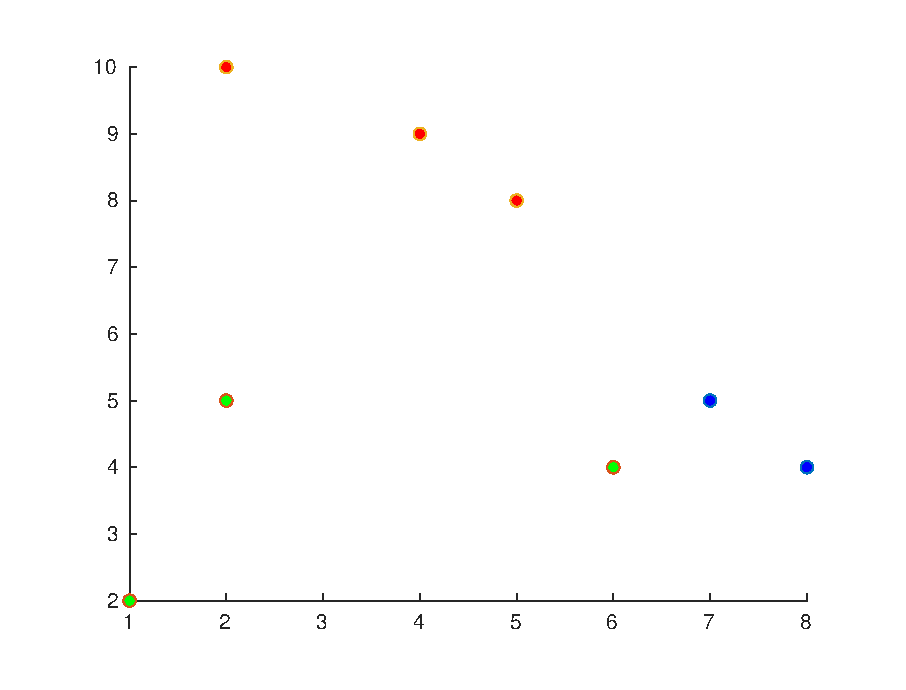
\includegraphics[width=\maxwidth{56.69844455594581em}]{figure_0.eps}
\end{center}

\begin{par}
\begin{flushleft}
Compute the new \texttt{Y:}
\end{flushleft}
\end{par}

\begin{matlabcode}
for i=1:3
    ci = D(:,3) == i;
    x = mean(D(ci,1));
    y = mean(D(ci,2));
    Y(i,:)=[x,y];
end
Y
\end{matlabcode}
\begin{matlaboutput}
Y = 3x2    
    7.5000    4.5000
    3.0000    3.6667
    3.6667    9.0000

\end{matlaboutput}

\begin{par}
\begin{flushleft}
Repeat the process:
\end{flushleft}
\end{par}

\begin{matlabcode}
%Distances
for j=1:3
    for i=1:8
        dist(i,j)=distance(D(i,1:2),Y(j,:),2);
    end
end
dist
\end{matlabcode}
\begin{matlaboutput}
dist = 8x3    
    7.7782    6.4118    1.9437
    5.5227    1.6667    4.3333
    0.7071    5.0111    6.6165
    4.3012    4.7726    1.6667
    0.7071    4.2164    5.2068
    1.5811    3.0185    5.5176
    6.9642    2.6034    7.4907
    5.7009    5.4263    0.3333

\end{matlaboutput}
\begin{matlabcode}
%Assign
[v, idx] = min(dist, [], 2);
D(:,3) = idx;
%Plot
c1 = D(:,3) == 1
\end{matlabcode}
\begin{matlaboutput}
c1 = 8x1 logical array    
   0
   0
   1
   0
   1
   1
   0
   0

\end{matlaboutput}
\begin{matlabcode}
c2 = D(:,3) == 2;
c3 = D(:,3) == 3;
scatter(D(c1,1),D(c1,2), 'MarkerFaceColor', 'b');
hold on
scatter(Y(1,1),Y(1,2), 'MarkerFaceColor', 'b');
scatter(D(c2,1),D(c2,2), 'MarkerFaceColor', 'g');
scatter(Y(2,1),Y(2,2), 'MarkerFaceColor', 'g');
scatter(D(c3,1),D(c3,2), 'MarkerFaceColor', 'r');
scatter(Y(3,1),Y(3,2), 'MarkerFaceColor', 'r');
hold off
\end{matlabcode}
\begin{center}
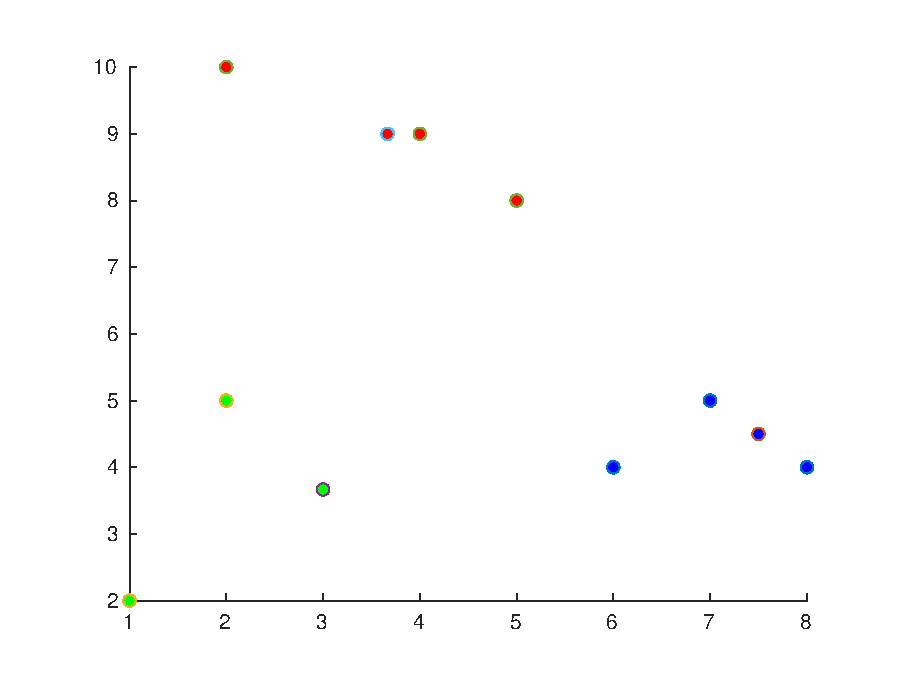
\includegraphics[width=\maxwidth{56.69844455594581em}]{figure_1.eps}
\end{center}
\begin{matlabcode}
%Optimize
for i=1:3
    ci = D(:,3) == i;
    x = mean(D(ci,1));
    y = mean(D(ci,2));
    Y(i,:)=[x,y];
end
Y
\end{matlabcode}
\begin{matlaboutput}
Y = 3x2    
    7.0000    4.3333
    1.5000    3.5000
    3.6667    9.0000

\end{matlaboutput}

\begin{par}
\begin{flushleft}
Again:
\end{flushleft}
\end{par}

\begin{matlabcode}
%Distances
for j=1:3
    for i=1:8
        dist(i,j)=distance(D(i,1:2),Y(j,:),2);
    end
end
dist
\end{matlabcode}
\begin{matlaboutput}
dist = 8x3    
    7.5572    6.5192    1.9437
    5.0442    1.5811    4.3333
    1.0541    6.5192    6.6165
    4.1767    5.7009    1.6667
    0.6667    5.7009    5.2068
    1.0541    4.5277    5.5176
    6.4377    1.5811    7.4907
    5.5478    6.0415    0.3333

\end{matlaboutput}
\begin{matlabcode}
%Assign
[v, idx] = min(dist, [], 2);
D(:,3) = idx;
%Plot
c1 = D(:,3) == 1
\end{matlabcode}
\begin{matlaboutput}
c1 = 8x1 logical array    
   0
   0
   1
   0
   1
   1
   0
   0

\end{matlaboutput}
\begin{matlabcode}
c2 = D(:,3) == 2;
c3 = D(:,3) == 3;
scatter(D(c1,1),D(c1,2), 'MarkerFaceColor', 'b');
hold on
scatter(Y(1,1),Y(1,2), 'MarkerFaceColor', 'b');
scatter(D(c2,1),D(c2,2), 'MarkerFaceColor', 'g');
scatter(Y(2,1),Y(2,2), 'MarkerFaceColor', 'g');
scatter(D(c3,1),D(c3,2), 'MarkerFaceColor', 'r');
scatter(Y(3,1),Y(3,2), 'MarkerFaceColor', 'r');
hold off
\end{matlabcode}
\begin{center}
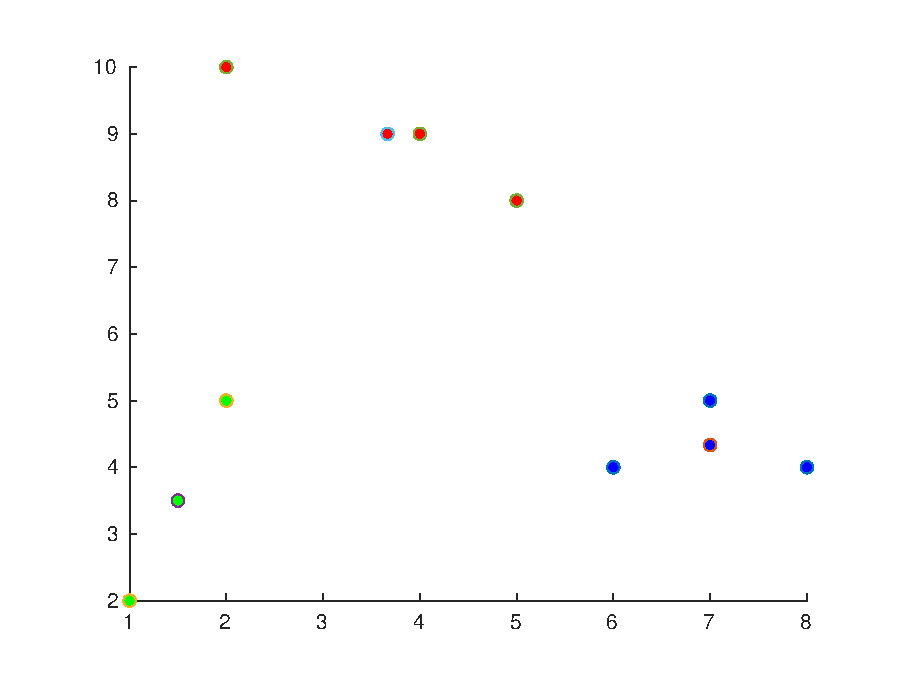
\includegraphics[width=\maxwidth{56.69844455594581em}]{figure_2.eps}
\end{center}
\begin{matlabcode}
%Optimize
for i=1:3
    ci = D(:,3) == i;
    x = mean(D(ci,1));
    y = mean(D(ci,2));
    Y(i,:)=[x,y];
end
Y
\end{matlabcode}
\begin{matlaboutput}
Y = 3x2    
    7.0000    4.3333
    1.5000    3.5000
    3.6667    9.0000

\end{matlaboutput}

\begin{par}
\begin{flushleft}
At this point we see how the clusters are the ones that we see naturally with our eyes. If we execute it again, we can see that the changes are very slight now:
\end{flushleft}
\end{par}

\begin{matlabcode}
%Distances
for j=1:3
    for i=1:8
        dist(i,j)=distance(D(i,1:2),Y(j,:),2);
    end
end
dist
\end{matlabcode}
\begin{matlaboutput}
dist = 8x3    
    7.5572    6.5192    1.9437
    5.0442    1.5811    4.3333
    1.0541    6.5192    6.6165
    4.1767    5.7009    1.6667
    0.6667    5.7009    5.2068
    1.0541    4.5277    5.5176
    6.4377    1.5811    7.4907
    5.5478    6.0415    0.3333

\end{matlaboutput}
\begin{matlabcode}
%Assign
[v, idx] = min(dist, [], 2);
D(:,3) = idx;
%Plot
c1 = D(:,3) == 1
\end{matlabcode}
\begin{matlaboutput}
c1 = 8x1 logical array    
   0
   0
   1
   0
   1
   1
   0
   0

\end{matlaboutput}
\begin{matlabcode}
c2 = D(:,3) == 2;
c3 = D(:,3) == 3;
scatter(D(c1,1),D(c1,2), 'MarkerFaceColor', 'b');
hold on
scatter(Y(1,1),Y(1,2), 'MarkerFaceColor', 'b');
scatter(D(c2,1),D(c2,2), 'MarkerFaceColor', 'g');
scatter(Y(2,1),Y(2,2), 'MarkerFaceColor', 'g');
scatter(D(c3,1),D(c3,2), 'MarkerFaceColor', 'r');
scatter(Y(3,1),Y(3,2), 'MarkerFaceColor', 'r');
hold off
\end{matlabcode}
\begin{center}
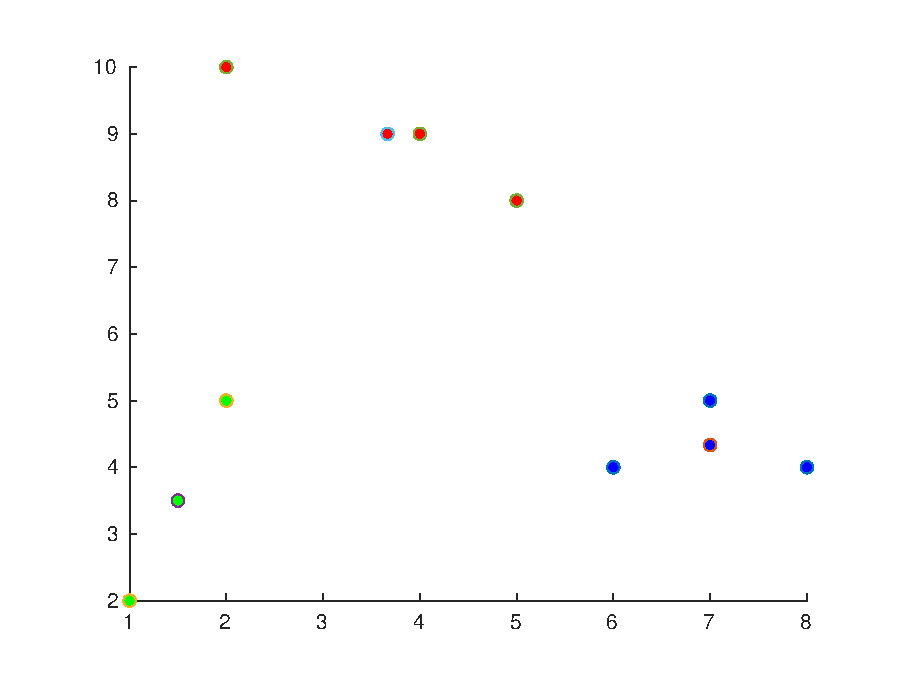
\includegraphics[width=\maxwidth{56.69844455594581em}]{figure_3.eps}
\end{center}
\begin{matlabcode}
%Optimize
for i=1:3
    ci = D(:,3) == i;
    x = mean(D(ci,1));
    y = mean(D(ci,2));
    Y(i,:)=[x,y];
end
Y
\end{matlabcode}
\begin{matlaboutput}
Y = 3x2    
    7.0000    4.3333
    1.5000    3.5000
    3.6667    9.0000

\end{matlaboutput}

\begin{par}
\begin{flushleft}
In fact, Y is not changing anymore!
\end{flushleft}
\end{par}


\matlabheadingthree{Functions}

\begin{par}
\hfill \break
\end{par}

\begin{matlabcode}
function d = distance(X, Y, m)
    n = length(X);
    d = 0;
    for i=1:n
        d = d + (X(i)-Y(i))^m;
    end
    d = sqrt(d);
end

\end{matlabcode}

\end{document}
